\documentclass[12pt,letterpaper,titlepage]{report}
\usepackage[latin1]{inputenc}
\usepackage{amsmath}
\usepackage{amsfonts}
\usepackage{amssymb}
\usepackage{graphicx}
\usepackage{pdfpages}
\usepackage{float}
\usepackage{titlesec}
\usepackage{needspace}
\usepackage{hyperref}
\usepackage{siunitx}
\usepackage[width=8.50in, height=11.00in, left=1.00in, right=1.00in, top=1.00in, bottom=1.00in]{geometry}
\usepackage[backend=bibtex,style=ieee]{biblatex}

% Default fixed font does not support bold face
\DeclareFixedFont{\ttb}{T1}{txtt}{bx}{n}{12} % for bold
\DeclareFixedFont{\ttm}{T1}{txtt}{m}{n}{12}  % for normal

% Custom colors
\usepackage{color}
\definecolor{deepblue}{rgb}{0,0,0.5}
\definecolor{deepred}{rgb}{0.6,0,0}
\definecolor{deepgreen}{rgb}{0,0.5,0}

\usepackage{listings}

% Python style for highlighting
\newcommand\pythonstyle{\lstset{
		language=Python,
		basicstyle=\ttm,
		otherkeywords={self},             % Add keywords here
		keywordstyle=\ttb\color{deepblue},
		emph={MyClass,__init__},          % Custom highlighting
		emphstyle=\ttb\color{deepred},    % Custom highlighting style
		stringstyle=\color{deepgreen},
		frame=tb,                         % Any extra options here
		showstringspaces=false            % 
}}

% Python environment
\lstnewenvironment{python}[1][]
{
	\pythonstyle
	\lstset{#1}
}
{}

% Python for external files
\newcommand\pythonexternal[2][]{{
		\pythonstyle
		\lstinputlisting[#1]{#2}}}

% Python for inline
\newcommand\pythoninline[1]{{\pythonstyle\lstinline!#1!}}

% Variables
\titleformat{\section}
{\needspace{8\baselineskip}\Large\bfseries}{\thesection}{1em}{}


% Document start ~~~~~~~~~~~~~~~~~~~~~~~~~~~~~~~~~~~~~~~~~~~~~~~~~~~~~~~~~~~~~~~~~~~~~~~~~~~~~~~~~~~~~

\title{Neural network-based controller}
\author{Justin Ng}
\bibliography{bib} 

\begin{document}
\pagenumbering{gobble}
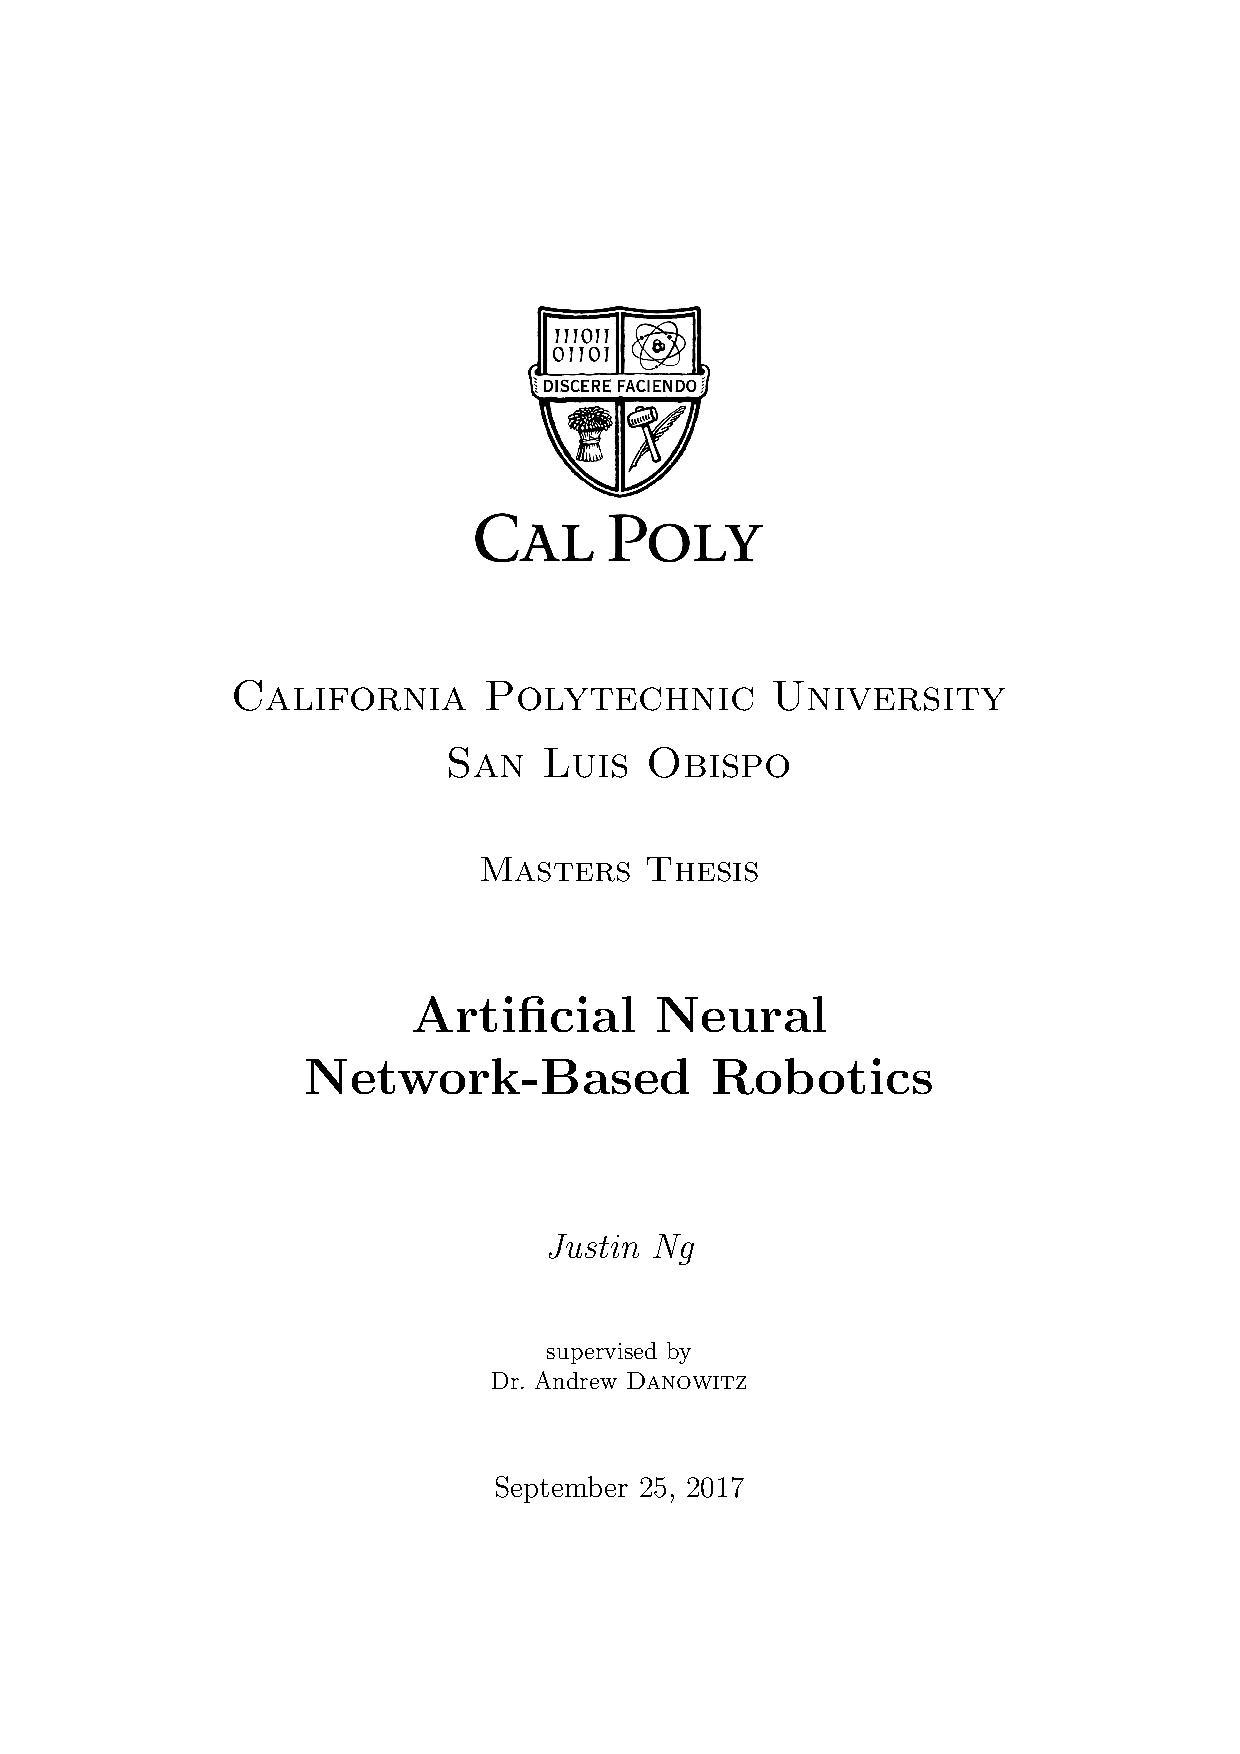
\includepdf{titlepage}
\newpage
\pagenumbering{roman}
\tableofcontents
\listoffigures
\listoftables


\chapter{\LaTeX\ Usage}

\section{Figures and Ref}
This is where I introduce stuff. See Figure \ref{fig:padthai}.

\begin{figure}[H]   % [h] means here
	\centering
	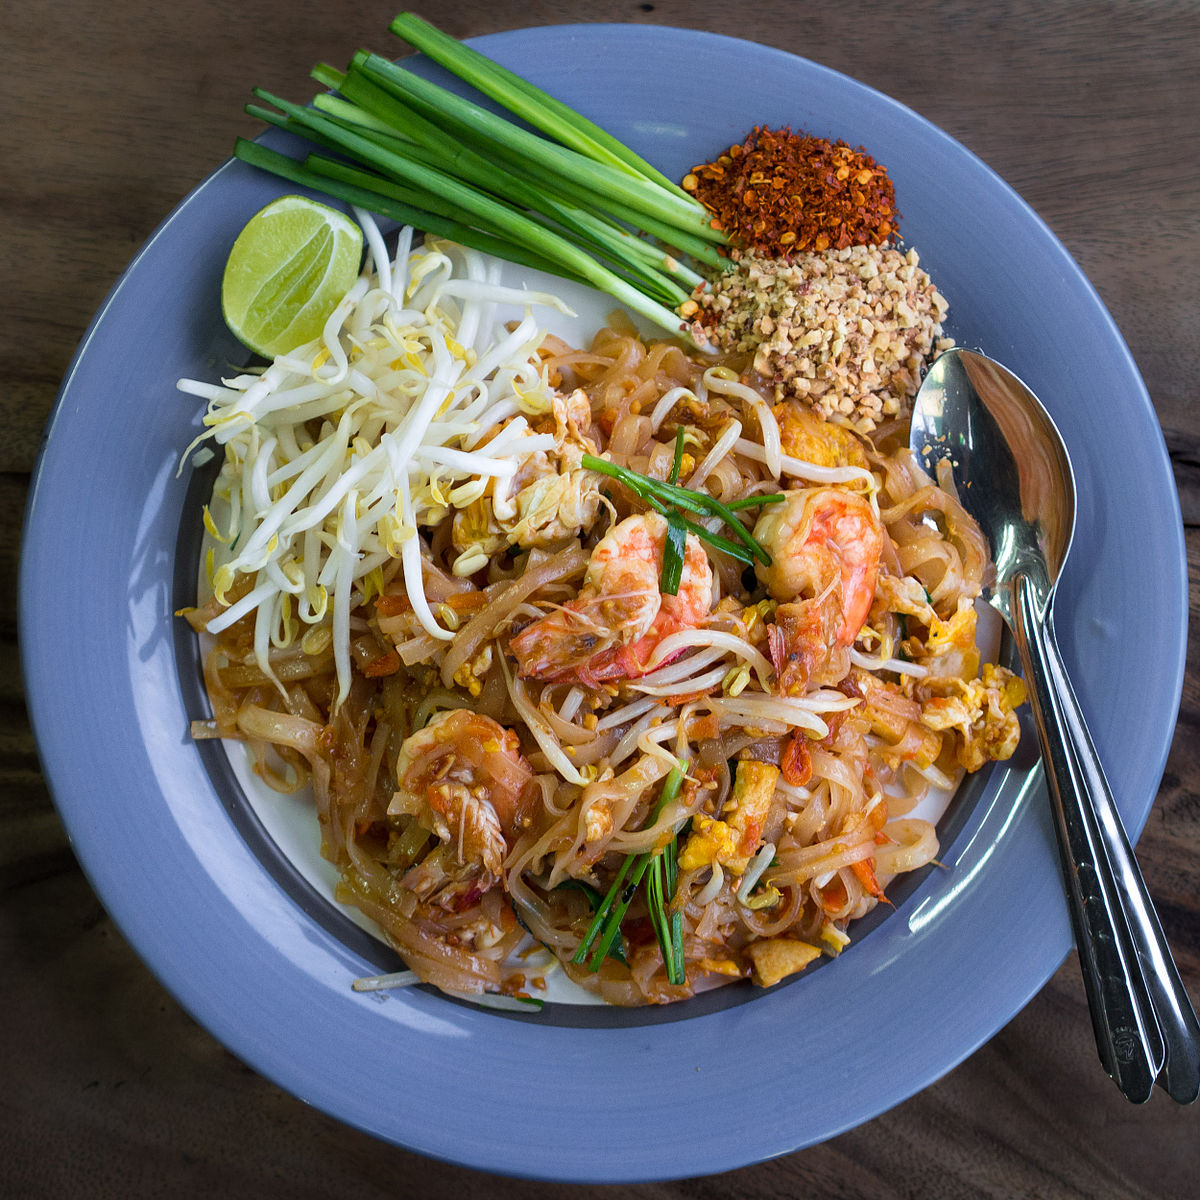
\includegraphics[width=3.6in]{images/padthai.jpg}
	\caption{Pad thai}
	\label{fig:padthai}
\end{figure}



\section{Math}

\begin{equation}
	f(x) = x^2
\end{equation}


This is an equation that we don't want to number: $$f(x) = x^2$$

Here's an in-line equation: $f(x) = x^2$.

Here's an aligned equation: Aligns at the \&.
\begin{align*}
	1 + 2 & = 3                       \\
	1     & = 3 - 2                   \\
	f(x)  & = x^2                     \\
	g(x)  & = \frac{1}{x}             \\
	F(x)  & = \int^a_b \frac{1}{3}x^3 \\
	\frac{1}{\sqrt{x}}
\end{align*}

\[\begin{bmatrix}
		a & \lambda \\
		c & d
	\end{bmatrix}\]



\section{Citations}


Random citation \autocite{nguyen_widrow_1990} embeddeed in text.

Random citation \autocite{DUMMY:1} embeddeed in text.

Random citation \autocite{nguyen_widrow_1990} embeddeed in text.
\autocite{negenborn_2003} \autocite{labbe_2017}

\section{Accents}

Premi\`ere	\.x

\section{Dashes}

The space is 3-dimensional.

Read pages 3--4.

I saw them---there were 3 men alive

The temperature dropped to $-$3 degrees.

\section{Lists}

\begin{itemize}
	\item  First Level
	      \begin{itemize}
		      \item  Second Level
		            \begin{itemize}
			            \item  Third Level
			                  \begin{itemize}
				                  \item  Fourth Level
			                  \end{itemize}
		            \end{itemize}
	      \end{itemize}
\end{itemize}
\begin{enumerate}
	\item First level item
	\item First level item
	      \begin{enumerate}
		      \item Second level item
		      \item Second level item
		            \begin{enumerate}
			            \item Third level item
			            \item Third level item
			                  \begin{enumerate}
				                  \item Fourth level item
				                  \item Fourth level item
			                  \end{enumerate}
		            \end{enumerate}
	      \end{enumerate}
\end{enumerate}

\section{Groups}
 {
  \hsize = 4 in
  \parindent = 0 pt
  \leftskip = 1 in
  will produce a paragraph that is four
  (this is an easy mistake to make).
  \par
 }


\section{Code highlighting}

\begin{python}
	class MyClass(Yourclass):
	def __init__(self, my, yours):
	bla = '5 1 2 3 4'
	print bla
\end{python}


\end{document}